% Drawing 152/01-6 -- folder 152, batch 01, archive page 1 (PDF page 2).
% Transcription: en haut, au milieu : une ligne horizontale portant cinq sommets $s_0$, $s_1$, $s_2$, $s_3$, $s_4$, fléchée entre eux ; sur chaque sommet, un bouquet de boucles en pétales (une sur $s_0$, trois sur $s_1$, deux sur $s_2$, trois sur $s_3$, trois sur $s_4$), chacune marquée « $w$ » ; « $w$ » encore sous les arêtes $s_1 s_2$ et $s_2 s_3$. Au-dessous de $s_0$, une petite figure : une boucle sur un sommet relié par une arête à un second sommet.
% Kind: chain of five vertices with bouquets of loops marked w. Method 2 (schematic redraw from the facsimile). Status: ok.
% Notes: The line through the five vertices (points), with arrowheads as on the page: from s_0 to s_1, from s_2 to s_1, from s_3 to s_2, from s_3 to s_4; on each vertex its loops, drawn as petals from the vertex (1, 3, 2, 3, 3), a letter w above each petal and under the two middle edges; the labels s_0 to s_4 under the vertices. Below s_0 the small figure: a loop on a vertex, and an edge from it to a second vertex. Overlaid on the 400 dpi colour facsimile on 2026-11-12 (Opus 5.5) and corrected: the earlier redraw stood 1 to 2 mm off (vertices s_0, s_1 and s_4 to the left and low, petals too narrow and shifted); the five vertices are now placed where the strokes meet, the line drawn through them, each petal redrawn from its own outline (its width, tip and lean as on the page) and the arrowheads and labels moved with them. At 400 dpi the loops are clear: one on s_0, three on s_1 (the third with a doubled outline), two on s_2, three on s_3, three on s_4. The isolated heavy point under the small figure is drawn, as on the page; whether it belongs to that figure is not known. Redrawn 2026-11-12 (issue 128): to check again.
% Coordinates: 1 unit = 1 mm = 1/100 of the crop width (bbox in page fractions: [0.33, 0.075, 0.6, 0.215]).
% Redrawn by Claude (claude-fable-5-2), issue #128, 2026-11-12; not checked by a human; not compiled (no TeX in the session).
% Corrected by Claude (claude-opus-5-5) 2026-11-12 (issue #128): overlaid on the 400 dpi colour facsimile and corrected from it. Not compiled. Status: ok.
% Rights: reproduces part of the work -- behind RENDER_TRANSCRIPTS, never published by itself.
\documentclass[tikz,border=3pt]{standalone}
\usepackage{amsmath,amssymb}
\usetikzlibrary{patterns,arrows.meta}
\tikzset{pencil/.style={black!45}, struck/.style={black!35}, mpt/.style={circle,draw,inner sep=1.3pt}, pt/.style={circle,fill,inner sep=0.9pt}, opt/.style={circle,draw,fill=white,inner sep=1.1pt}}
\begin{document}
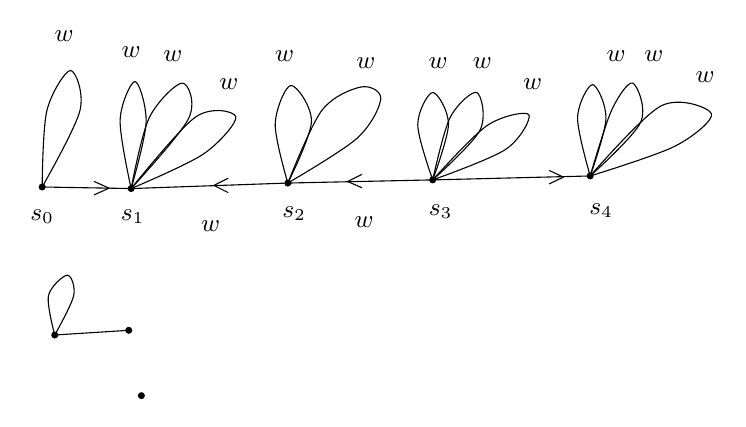
\begin{tikzpicture}[x=1mm,y=1mm,line cap=round,line join=round,font=\scriptsize]
\draw (6,-24.2) -- (17.3,-24.4) -- (37.2,-23.7) -- (55.6,-23.3) -- (75.6,-22.8);
\node[pt] at (6,-24.2) {};
\node[pt] at (17.3,-24.4) {};
\node[pt] at (37.2,-23.7) {};
\node[pt] at (55.6,-23.3) {};
\node[pt] at (75.6,-22.8) {};
\draw (12.6,-23.5) -- (14.5,-24.35) -- (12.6,-25.2);
\draw (29.6,-24.9) -- (27.8,-24) -- (29.6,-23.1);
\draw (46.6,-24.3) -- (44.8,-23.5) -- (46.6,-22.6);
\draw (70.4,-22.1) -- (72.2,-22.95) -- (70.4,-23.8);
\draw plot[smooth, tension=0.55] coordinates {(6,-24.2) (10.8,-14.5) (9.6,-9.4) (6.6,-14.5) (6,-24.2)};
\draw plot[smooth, tension=0.55] coordinates {(17.3,-24.4) (19.2,-16) (17.8,-10.8) (15.9,-15.7) (17.3,-24.4)};
\draw plot[smooth, tension=0.55] coordinates {(17.3,-24.4) (24.6,-15.5) (23.8,-11) (19.6,-15.4) (17.3,-24.4)};
\draw plot[smooth, tension=0.55] coordinates {(17.3,-24.4) (26.5,-20) (30.6,-15.3) (25.5,-15.3) (17.3,-24.4)};
\draw plot[smooth, tension=0.55] coordinates {(37.2,-23.7) (40.2,-15.9) (37.6,-11.3) (35.6,-16.2) (37.2,-23.7)};
\draw plot[smooth, tension=0.55] coordinates {(37.2,-23.7) (46,-18) (49,-13) (46.5,-11.5) (41.5,-14.5) (37.2,-23.7)};
\draw plot[smooth, tension=0.55] coordinates {(55.6,-23.3) (57.6,-16.2) (55.6,-12.2) (53.7,-16.3) (55.6,-23.3)};
\draw plot[smooth, tension=0.55] coordinates {(55.6,-23.3) (61.6,-17) (61.2,-12.2) (57.8,-15.4) (55.6,-23.3)};
\draw plot[smooth, tension=0.55] coordinates {(55.6,-23.3) (64.9,-19.4) (67.8,-15) (62.5,-16.4) (55.6,-23.3)};
\draw plot[smooth, tension=0.55] coordinates {(75.6,-22.8) (77.6,-15.5) (75.9,-11.2) (74,-15.4) (75.6,-22.8)};
\draw plot[smooth, tension=0.55] coordinates {(75.6,-22.8) (82,-16) (81,-11) (78.3,-14.5) (75.6,-22.8)};
\draw plot[smooth, tension=0.55] coordinates {(75.6,-22.8) (86.4,-19) (91,-14.9) (84.6,-13.9) (75.6,-22.8)};
\node[inner sep=1pt] at (8.8,-5) {\small $w$};
\node[inner sep=1pt] at (17.3,-7.1) {\small $w$};
\node[inner sep=1pt] at (22.6,-7.6) {\small $w$};
\node[inner sep=1pt] at (29.7,-11.1) {\small $w$};
\node[inner sep=1pt] at (36.8,-7.6) {\small $w$};
\node[inner sep=1pt] at (47.1,-8.5) {\small $w$};
\node[inner sep=1pt] at (56.3,-8.5) {\small $w$};
\node[inner sep=1pt] at (61.9,-8.5) {\small $w$};
\node[inner sep=1pt] at (68.3,-11.1) {\small $w$};
\node[inner sep=1pt] at (78.9,-7.6) {\small $w$};
\node[inner sep=1pt] at (83.7,-7.6) {\small $w$};
\node[inner sep=1pt] at (90.2,-10.3) {\small $w$};
\node[inner sep=1pt] at (27.4,-29.2) {\small $w$};
\node[inner sep=1pt] at (46.9,-28.7) {\small $w$};
\node[inner sep=1pt] at (6,-28) {\small $s_{0}$};
\node[inner sep=1pt] at (17.5,-28) {\small $s_{1}$};
\node[inner sep=1pt] at (38,-27.6) {\small $s_{2}$};
\node[inner sep=1pt] at (56.6,-27.3) {\small $s_{3}$};
\node[inner sep=1pt] at (77,-27.2) {\small $s_{4}$};
\draw plot[smooth, tension=0.55] coordinates {(7.6,-43) (10,-38) (9.2,-35.4) (6.8,-38) (7.6,-43)};
\draw (7.6,-43) -- (17,-42.4);
\node[pt] at (7.6,-43) {};
\node[pt] at (17,-42.4) {};
\node[pt] at (18.6,-50.7) {};
\end{tikzpicture}
\end{document}
